\documentclass{article}
 
\usepackage{hyperref}
\usepackage{url}
\usepackage{float}
\usepackage{graphicx}
 
\graphicspath{ {./images/} }
 
\title{Article 3 Reference Critic}
 
\author{Nikolai Perlt}
 
\date{December 2020}
 
\begin{document}
 \maketitle
\section*{Intro}
In this report I will try to further improve on the excellent report Quick-Sort Performance written by Michael Ejdal Lundsgaard\cite{pythonVsCSQuickSort}. I will do this by finding references that I believe would help improve the article, and further validate the point the original author wanted to make. 
 
\section*{C\# versus Python runtime operations}
% TODO: mention and link the actual article.
% 1 What will this reference help the article.
In the original article the author concluded that C\# is 14x faster than Python. However, this is only when comparing C\# and Python on quick sort algorithm. Is this still applicable when compared to other algorithms, or other forms of computer operations. If the article had references another article also concluding this, it would further strengthen the statement that C\# is a significantly faster language than Python. To this I have found an article that I believe accomplishes this purpose\cite{karaci2015performance}. 
% 2 What does this reference actually say
 
The article measures on multiple different runtime metrics of C\# and python. The ones I will discuss and compare to the original article are.
 
\begin{itemize}
 \item Sorting 10000 elements with selection sort.
 \item Multiplication of two matrices.
 \item Printing Hello World on the screen 5000 times. 
\end{itemize}
\begin{figure}
 \caption{Runtime comparison}
 \label{fig:runtimeTable}
 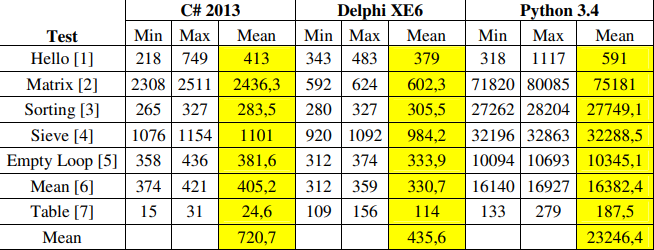
\includegraphics[width=\textwidth]{runtimeTable.png}
\end{figure}
The main aspect I would focus on in the reference article, is sorting since it is the driving force of the original article. We can see from table\ref{fig:runtimeTable} taken from the reference article, that the reference article as well can conclude that sorting is magnitudes faster using C\# instead of Python. This would have further solidified the main point of the original article, that C\# is faster than Python when comparing sorting algorithms. Not only that, but also that this is not only true for quick sort, but other sorting algorithms as well.
 
I also believe the article could benefit from quickly mentioning the remaining two metrics. These are still measurably faster when using C\#, however still not on the same scale as sorting. By showing the reader this aspect, it would supplementary show C\# speed advantage is not only applicable to sorting but also other forms of operations. This would in turn make the article more usable to more readers.
% 3 What are some variables to keep in mind when using the reference.
There are some aspects to keep in mind when comparing the original article with the reference article. The original article never mentions what version of Python nor C\# it is running. Since the Original article was written in 2020, and the reference article was written in 2015, it is a very real possibility that we are comparing two different versions of the languages. This could mean that Python has lowered the gap between the two languages, thereby making the comparison between the two articles not as precise.
 
\section*{PyPy}
% How would referencing pypy further help the article
%   * Pypy is often mentioned in the article and a lot of statements are made that %are not backed up by references.
 
% The article does not state anything that is not true, however still citing a reference would add more credibility to the article.
The author not only compares Python to C\#, but also PyPy, and throughout the article some statements about PyPy are made that i believe could use sources. Some of these statements are
\begin{itemize}
 \item PyPy being a JIT compiler.
 \item That PyPy does not have any benefits on the first run through of the code.
\end{itemize}
These statements are never backed up by sources, but by using a source such as\cite{pypy}, the reader would be left without a doubt as to the validity of the claims. None of the statements are false, however by having external sources backing up the claims it would further cement the article as reputable.
 
\section*{Outro}
Overall I think this is an incredible article written by Michael Ejdal Lundsgaard. It's an interesting topic that is well explained and well documented. However, I believe that if the two references mentioned in this critic could be incorporated, it would even further improve the quality of the article.
 
 
\bibliographystyle{unsrt}
\bibliography{references}
 
\end{document}

